\documentclass[a4paper]{article}
\usepackage[letterpaper, margin=1in]{geometry} % page format
\usepackage{listings} % this package is for including code
\usepackage{graphicx} % this package is for including figures
\usepackage{amsmath}  % this package is for math and matrices
\usepackage{amsfonts} % this package is for math fonts
\usepackage{tikz} % for drawings
\usepackage{hyperref} % for urls
\usepackage{stackengine}

\newcommand\tab[1][0.5cm]{\hspace*{#1}}
\newcommand{\floor}[1]{\lfloor #1 \rfloor}

\title{Homework 3}
\author{Kaitlyn Mulligan}
\date{5/1/19}

\begin{document}
\lstset{language=Python}

\maketitle

\section{Instructions}
This assignment could be written in \LaTeX, just as the last homework assignment. Write in 
understandable, easy to follow English. Make sure you provide good illustrations and figures; 
\textbf{however, do not just throw in figures without a proper explanation and discussion.  
Figures are meant to prove a point you are making verbally; figures are a resource and not 
the main point.}  Remember to include your Python programs in your assignment (\textbf{in 
GitHub only please}).\\
\tab Your assignment should be submitted in two ways: through GitHub, and in hardcopy (in class).  
Use the \textbf{same} repository you have been using and submit your work in a folder named 
"\verb|lastname-xx|", where lastname is your last name xx is the number of the assignment.

% ----------------------------------------------------------------------------------------------

\section{Problem Set}
The following is a list of problems you will work on. When providing your solutions (hopefully 
using \LaTeX), do not simply give the final answer, show how you arrived to the solution, justify 
your assumptions, and explain your results clearly.

% ----------------------------------------------------------------------------------------------

\subsection{1} Use \verb|sklearn|’s implementation of $k$-Nearest Neighbors for regression 
purposes, which is found in \\
\verb|sklearn.neighbors.KNeighborsRegressor|.  You will find the best value of $k$ using 10-fold 
CrossValidation (CV), which is found in \verb|sklearn.model_selection.KFold|.
\begin{itemize}
    \item[(a)] You will modify the python code below to generate 1000 data points, or alternatively 
    you could use part of your semester project dataset if it is related to regression.
    \lstinputlisting[language=Python,frame=single]{hw3_1_a_gendata.py}
    
    \textbf{Solution:} To modify the python code above to generate 1000 data points you can change 
    the line that says ``\verb|x, y, ytrue = genDataSet(100)|" to ``\verb|x, y, ytrue = genDataSet(1000)|".  
    This modified code can be found in the section labeled \verb|Question 1 part a| of the 
    \verb|homework3.py| file in GitHub.  Running this code results in the following plot:
    \begin{center}
        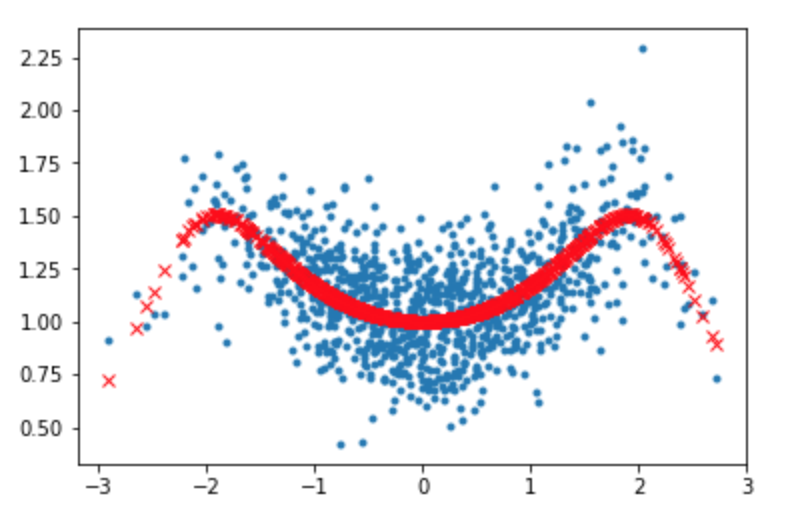
\includegraphics[width=0.6\textwidth]{1a.jpg}
    \end{center}
    This graph shows the true values of y in red and the noisy values of y in blue.
    
    \item[(b)] Using 10-fold CV, you will report the three best values of $k$-neighbors that yield 
    the best CV $E_{\text{out}}$.  You will vary the values of $k$ in the following range: $k = 1, 
    3, 5, \ldots, 2 \lfloor\frac{N+1}{2}\rfloor - 1$.
    
    \textbf{Solution:} The following plot shows the values of $k$ in the range of $k = 1, 3, 5, 
    \ldots, 2 \lfloor\frac{N+1}{2}\rfloor - 1$ with their respective values of $E_{\text{out}}$ 
    represented as \verb|msek[k]| using 10-fold CV.
    \begin{center}
        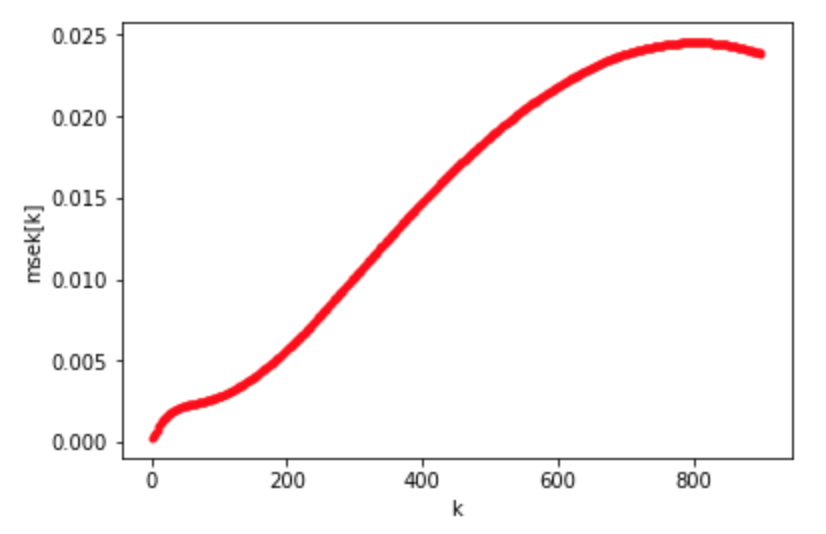
\includegraphics[width=0.6\textwidth]{1b.jpg}
    \end{center}
    The three best values $k$-neighbors that yield the best CV $E_{\text{out}}$ are $k = 1.0, 3.0,$ 
    and $5.0$ with CV $E_{\text{out}}$ values of $0.0003854796498389614, 0.0004521421202428154,$ and 
    $0.0005609831735528213$, respectively.

    \item[(c)] You will report the best CV $E_{\text{out}}$.
    
    \textbf{Solution:} The program reports that the best CV $E_{\text{out}}$ is $0.0003854796498389614$ 
    and occurs when $k = 1.0$.  The code that found this result can be found at the bottom of the 
    section of code labeled \verb|Question 1 part b and c| in the \verb|homework3.py| file in GitHub.
\end{itemize}

% ----------------------------------------------------------------------------------------------

\subsection{2}  (extra credit) Using the same dataset you just tried in the previous problem, 
repeat the experiment 100 times storing the best three $k$ number of neighbors in every single 
trial, and at the end of all trials plot a histogram of all the values of $k$ that you saved.

\textbf{Solution:} After repeating the experiment 100 times, I stored the best three $k$ number 
of neighbors in every single trial.  I then plotted a histogram of all the values of $k$ that 
were saved.  The code that stored the values of $k$ as well as plotting the histogram can be found 
in a section labeled \verb|Question 2| and \verb|Question 2 Plot| in the \verb|homework3.py| file 
in GitHub.  Below is the histogram it produced.
\begin{center}
    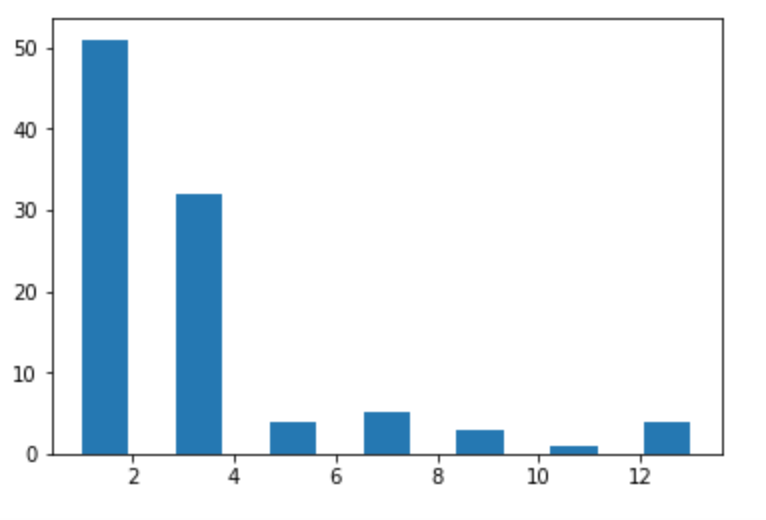
\includegraphics[width=0.6\textwidth]{2.jpg}
\end{center}

% ----------------------------------------------------------------------------------------------

\subsection{3} \textbf{Experiment with k-means for color quantization.}\\
Using sklearn’s implementation of $k$-means, find the best color clustering for an image of your 
choice. \textit{A good portrait of yourself could be fun (just sayin’)}.  Color quantization is 
the science behind compression of images. The idea is to represent an image with fewer colors 
than the original. The experiment consists of the following steps:
\begin{itemize}
    \item[(a)] Download to your computer the file \verb|hw3.kmeans.img.py|
    
    \textbf{Solution:} I downloaded the file to my computer and then pasted it into my Google 
    Colab for this homework assignment in a section labeled \verb|Question 3| in the \verb|homework3.py| 
    file in GitHub.
    
    \item[(b)] In the same folder where you downloaded the program, save a copy of your picture 
    for experimentation.

    \textbf{Solution:} In the same folder in which I downloaded the program, I saved a copy 
    of the picture I am going to use for experimentation.  In addition, I also uploaded it to 
    my Google Colab so I could run the program there.  For this exercise, I decided to use a 
    picture I took the last time I went to a Yankee game.

    \item[(c)] Go to line 23 and set \verb|n_colors| with your choice of a number of colors 
    between 2 and 64. This number is actually the number of clusters (or $k$) we are searching 
    for in an unsupervised manner using $k$-means.
    
    \textbf{Solution:} In line 23 of the program, I decided to set \verb|n_colors| to 64 to 
    start off with.
    
    \item[(d)]  Then go to line 25 and replace the image file name with the name of \textbf{your} 
    image file. This is where your image is read into a numpy array.

    \textbf{Solution:} In line 25 of the program, I replaced the image file name with the name of 
    my image file, \verb|yankees.jpg|.

    \item[(e)] Run the program. Observe the result.  If the result does not look funny to you, 
    repeat from 3.(c) until it does. Then, report your result image along with your answers to 
    the following questions:
    \begin{itemize}
        \item[(i)] Explain $\ldots$ what happens when you increase or decrease the value of 
        \verb|n_colors|?
        \item[(ii)] Explain $\ldots$ in what other possible applications do you think this 
        can be useful?
        \item[(iii)] Why do you think the resulting picture was funny at the end?
    \end{itemize}

    \textbf{Solution:} After running the program first with \verb|n_colors| set equal to 64, 
    I decided to keep running the program, dividing the colors by two each time until \verb|n_colors| 
    equaled 4.  Below are my results with the first picture being the original picture.\\
    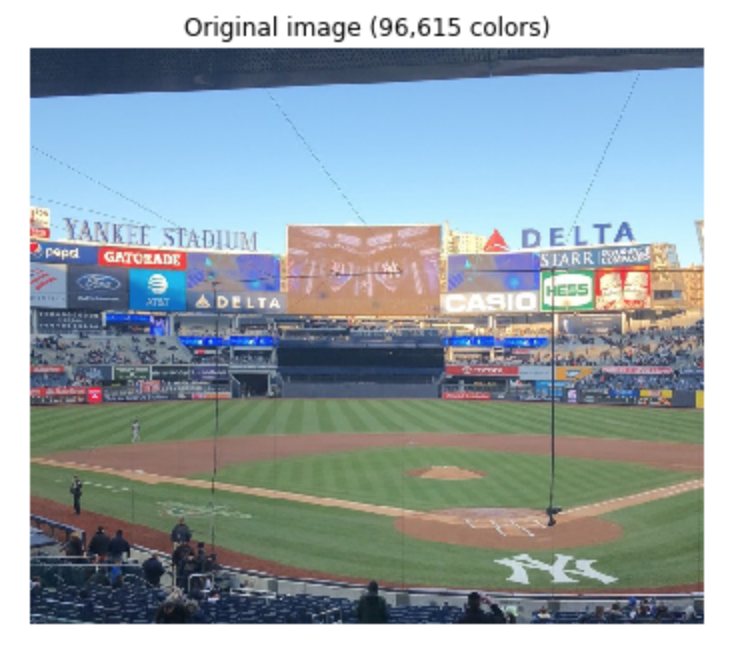
\includegraphics[width=0.5\textwidth]{original.jpg}
    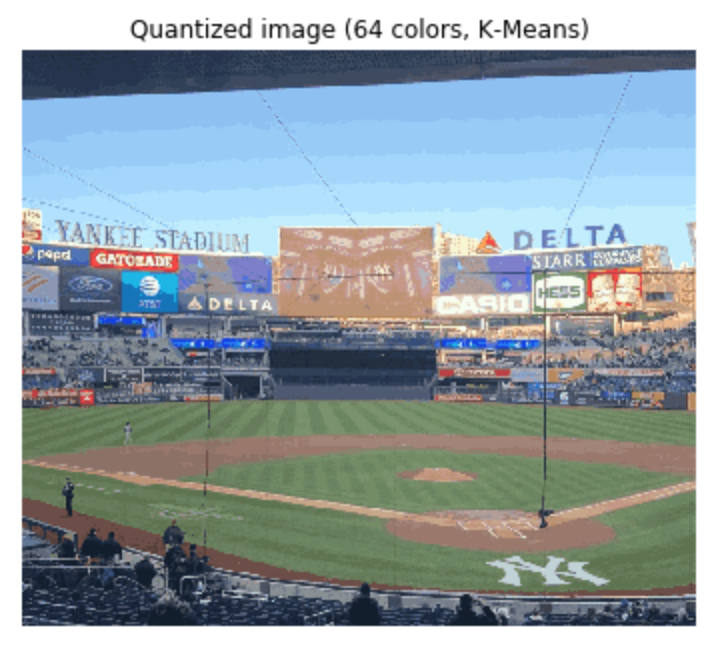
\includegraphics[width=0.49\textwidth]{64colors.jpg}\\
    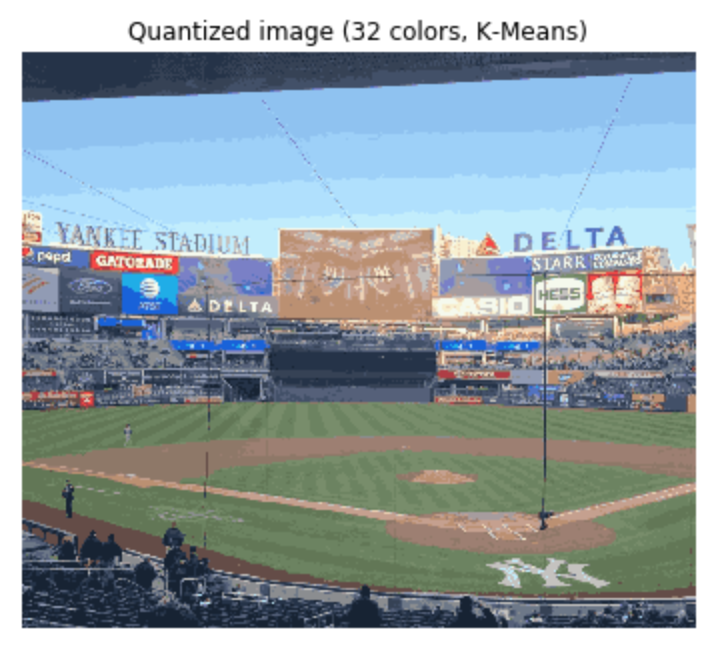
\includegraphics[width=0.5\textwidth]{32colors.jpg}
    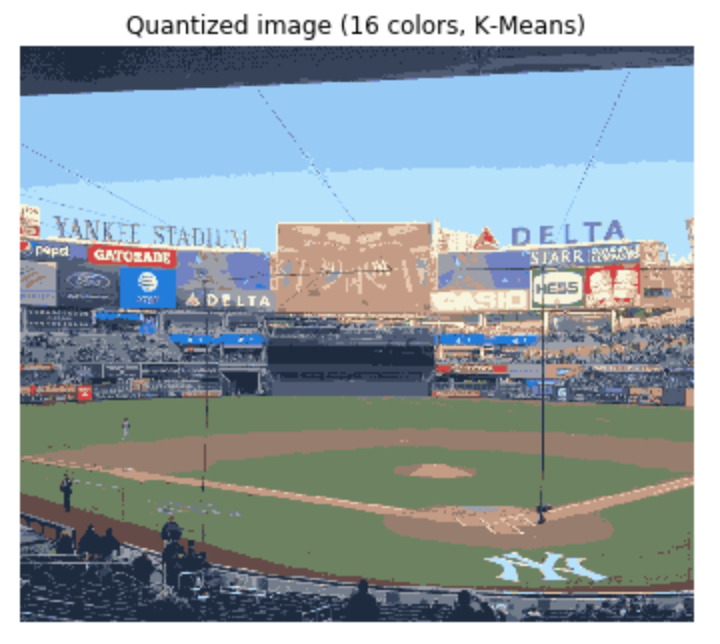
\includegraphics[width=0.5\textwidth]{16colors.jpg}\\
    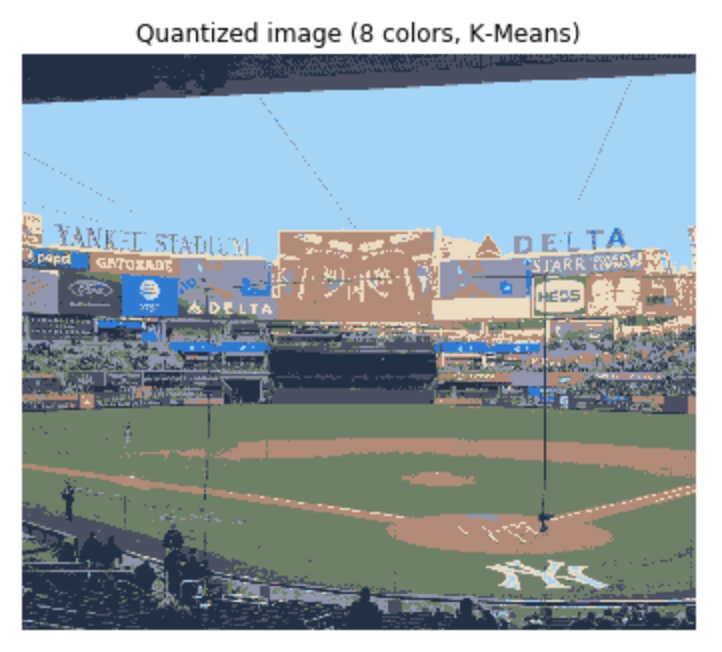
\includegraphics[width=0.5\textwidth]{8colors.jpg}
    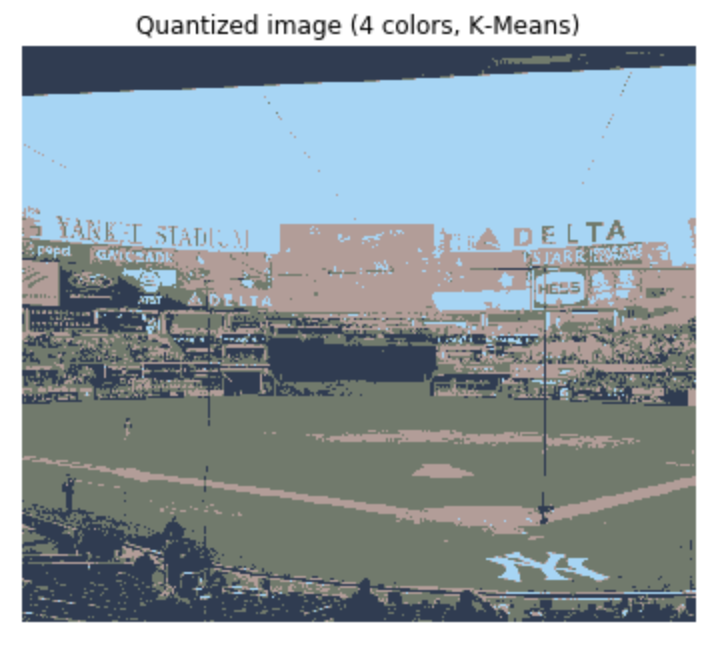
\includegraphics[width=0.5\textwidth]{4colors.jpg}
    \begin{itemize}
        \item[(i)] When you increase the value of \verb|n_colors| you are increasing the number 
        of clusters (or $k$) we are searching for in an unsupervised manner using $k$-means.  
        On the other hand when you decrease the value of \verb|n_colors| you are decreasing the 
        number of clusters (or $k$) we are searching for in an unsupervised manner using $k$-means.  
        This means when we increase \verb|n_colors|, we are allowing more clusters of different 
        colors.  When we decrease \verb|n_colors|, we are using less clusters of different colors.  
        Therefore, when we use \verb|n_colors| equal to 64, we are allowing 64 different colors so 
        it looks closer to the original image.  When we continuously decrease \verb|n_colors| all 
        the way down to 4, we are having it produce the same image, but with only 4 colors.
        \item[(ii)] This process can be useful if a program has memory limitations in which it 
        can only support a limited number of colors.  This can also be used in cases where there 
        are small dimensions and we want to learn what groups form naturally in the data.
        \item[(iii)] The resulting picture at the end is funny because there are only 4 colors 
        present in the image.  The original image started with 96,615 colors.  When the image 
        had 64 colors uing $k$-means, it still looked fairly similar to the original picture.  
        After cutting down the number of colors all the way down to 4, we are only letting it 
        produce a picture with 4 colors using $k$-means.
    \end{itemize}
\end{itemize}

% ----------------------------------------------------------------------------------------------

\subsection{4} \textbf{Neural networks: The MLP}
\begin{itemize}
    \item[(a)] Download the python program \verb|hw3.MLP.sol.py| which implements a 10-fold 
    cross-validation approach to find the best number of neurons and the best learning parameter 
    $\eta$ (eta) in an MLP for regression. For learning purposes you could download \verb|hw3.MLP.py| 
    first, which is a simple implementation of the MLP.
    
    \textbf{Solution:} I downloaded both \verb|hw3.MLP.sol.py| and \verb|hw3.MLP.py| to later 
    implement in order to find the best number of neurons and the best learning parameter $\eta$ 
    in an MLP for regression.  I then copied \verb|hw3.MLP.py| into Google Colab.  This can be seen 
    in the section labeled \verb|Question 4 - MLP|, subsection \verb|4a| in my \verb|homework3.py| in GitHub.  
    To begin understanding the MLP, I ran the simple implementation with 1000 data points.  I obtained 
    the following output, where, the noisy input is blue, the MLP is black, and the actual values 
    are red.
    \begin{center}
        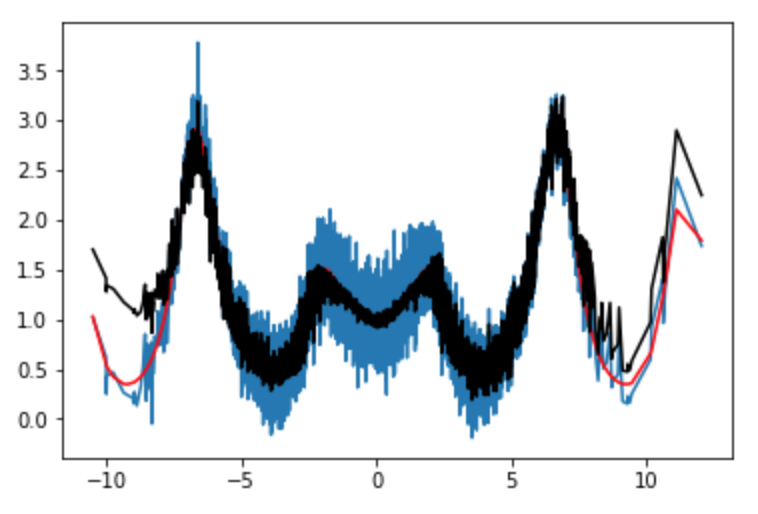
\includegraphics[width=0.6\textwidth]{4a1000.jpg}
    \end{center}
    
    \item[(b)] Download the python program \verb|hw3_4_a_gendata.py| which generates random data.
    
    \textbf{Solution:} I downloaded the program \verb|hw3_4_a_gendata.py| as well as uploaded 
    it to Google Colab so that random data will be generated when I run the program.
    
    \item[(c)] Run the program in 4.(a) for 1,000 samples, and then take note of the best number 
    of neurons and $\eta$. Go here \verb|https://goo.gl/forms/QFmaNWYaFLcPWdim2| and report your 
    results. You can do it as many times as you want, but at least one is required.
    
    \textbf{Solution:} Running the program in 4.(a), I used the program \verb|hw3.MLP.sol.py| in 
    Google Colab in the section labeled \verb|Question 4 c)|.  I set $N$ equal to 1000 for 1000 
    samples.  After the program finished, it reported that the best number of neurons was 36 with 
    $\eta = 0.2$.  This gave a testing set CV score of -1.785874.  Below is the output I obtained.
    \begin{center}
        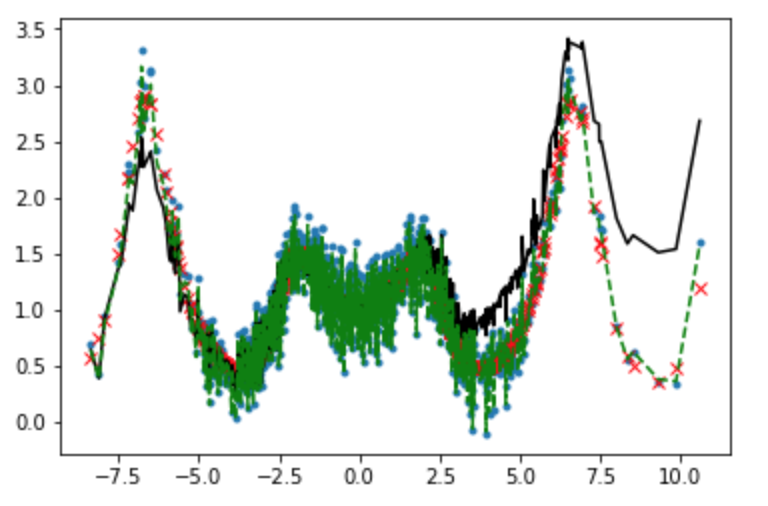
\includegraphics[width=0.6\textwidth]{4c.jpg}
    \end{center}
    
    \item[(d)] \textbf{Explain} your results. What do you think is happening? What is your 
    interpretation of the number of neurons with respect to the performance of the network?
    
    \textbf{Solution:} While analyzing this graph, note that our prediction is represented in black, 
    the green represents the prediction using linear regression, red is the best solution, and 
    blue is the output.  Viewing the graph we obtained here, it seems that our prediction was doing 
    fairly well until the end when it kind of diverged from the rest slightly.  When looking at the 
    output of the program, we want the value of the CV score to be larger.  As we can see in the output, 
    every time the program output a new value for neurons and $\eta$, it had the value of the CV score 
    increase.  Therefore, as stated in part (c) we have that having 36 neurons and $\eta = 0.1$ produced 
    the largest CV score with 1,000 samples.  As we can see, we need not too few neurons, but also not 
    too many.  If we have too many neurons the program will overfit, but the cross validation in this 
    program will catch that for us.  The value of $\eta$ was fairly consistent at $\eta = 0.1$.

    \item[(e)] (\textbf{extra credit}) Repeat 4.(c)-(d) but for 10,000 samples.
    
    \textbf{Solution:} I first repeated 4.(a) to see what that output would look like compared 
    to the one using 1.000 samples.  Below is the graph I obtained from this part.
    \begin{center}
        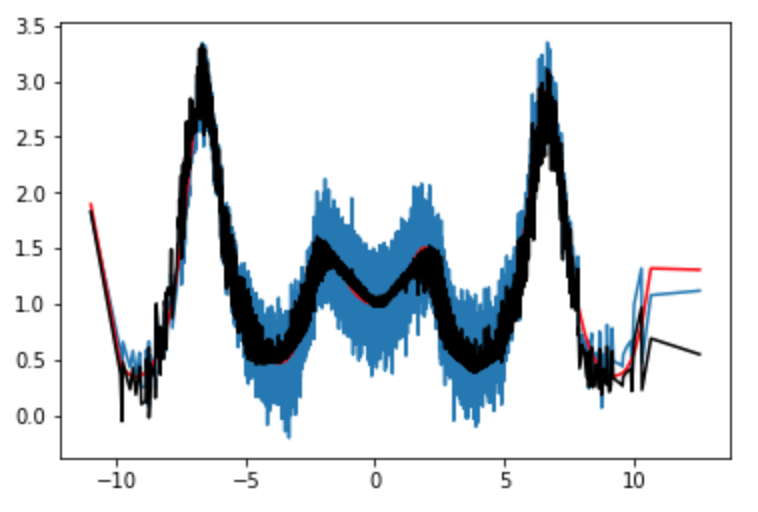
\includegraphics[width=0.6\textwidth]{4e-a10000.jpg}
    \end{center}
    I then repeated 4.(c)-(d) with 10,000 samples instead of 1,000 samples.  After running 
    this program, it reported that the best number of neurons was 50 with $\eta = 0.1$.  This 
    gave a testing set CV score of -1.385268.  Below is the output I obtained.
    \begin{center}
        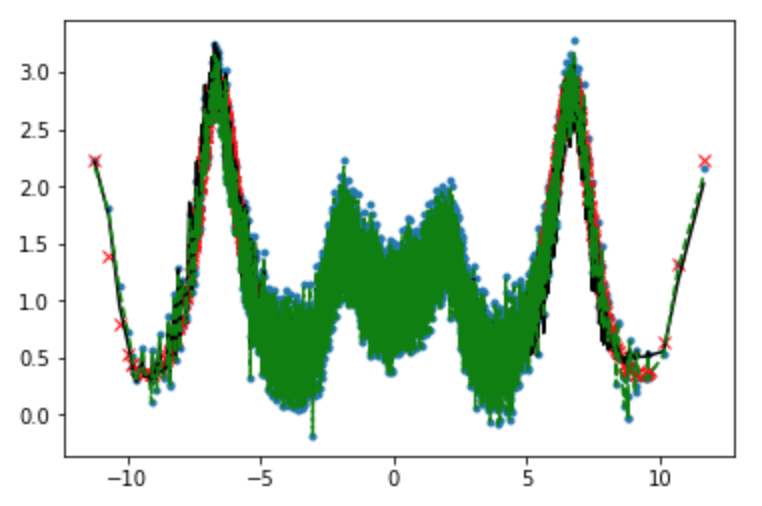
\includegraphics[width=0.6\textwidth]{4e-c.jpg}
    \end{center}
    As stated in part (d), while analyzing this graph, note that our prediction is represented in 
    black, the green represents the prediction using linear regression, red is the best solution, 
    and blue is the output.  Viewing the graph here, now with 10,000 samples, our prediction has 
    stayed with the green, red, and blue pretty well.  Compared to the graph obtained with 1,000 
    samples, our solution here seems to have a better prediction that stays with the linear regression, 
    the best solution, and the output.  Again, looking at the neurons, value of $\eta$, and the CV score, 
    we want the value of the CV score to be larger.  As we can see as before, every time the program 
    output a new value for neurons and $\eta$, the value of the CV score increased.  Therefore, 
    as stated earlier, we have that for this program, with 10,000 samples, having 50 neurons and 
    $\eta = 0.1$ produced the largest CV score.  Here again, the value of $\eta$ was fairly consistent 
    at $\eta = 0.1$.  As stated above, we can see that we need not too few neurons, but also not 
    too many.  If we have too many neurons the program will overfit, but the cross validation in this 
    program will catch that for us.  Also, with larger sample sizes, the program may seem to use more 
    neurons.
\end{itemize}

\end{document}
